% =====================================================================
%  RidePool -- UML Sequence Diagram: one pooled ride, request to rating.
%  Endpoint paths and atomic function names are the real ones.
%  Standalone TikZ figure; pixel-like units match the SVG beside it.
%  It is TALL -- see the footer for placement.
% =====================================================================
\documentclass[border=4pt]{standalone}

\usepackage[T1]{fontenc}          % (*)
\usepackage{tikz}                 % (*)
\usetikzlibrary{arrows.meta}      % (*)
\usepackage{xcolor}               % (*)

\definecolor{riderblue}{HTML}{2563EB}
\definecolor{riderbg}{HTML}{EFF6FF}
\definecolor{inkdark}{HTML}{111827}
\definecolor{linegrey}{HTML}{374151}
\definecolor{midgrey}{HTML}{6B7280}
\definecolor{faintgrey}{HTML}{9CA3AF}
\definecolor{hairline}{HTML}{E5E7EB}
\definecolor{sunken}{HTML}{F9FAFB}
\definecolor{fragbg}{HTML}{F3F4F6}

\newcommand{\sqname}{\fontsize{5.4}{6.2}\selectfont\bfseries}
\newcommand{\sqrole}{\fontsize{4.2}{5.0}\selectfont}
\newcommand{\sqmsg}{\fontsize{4.8}{5.6}\selectfont}
\newcommand{\sqsub}{\fontsize{3.8}{4.6}\selectfont}
\newcommand{\sqphase}{\fontsize{5.2}{6.0}\selectfont\bfseries}
\newcommand{\sqfrag}{\fontsize{4.8}{5.6}\selectfont\bfseries}
\newcommand{\sqguard}{\fontsize{4.6}{5.4}\selectfont}

\tikzset{
  life/.style={draw=faintgrey, line width=0.35pt, dash pattern=on 1.4pt off 1.2pt},
  call/.style={draw=linegrey, line width=0.4pt, -{Stealth[length=1.5mm,width=1.1mm]}},
  ret/.style ={draw=linegrey, line width=0.4pt, dash pattern=on 1.6pt off 1.2pt,
               -{Stealth[length=1.5mm,width=1.1mm,open]}},
  asyn/.style={draw=linegrey, line width=0.4pt, -{Stealth[length=1.5mm,width=1.1mm,open]}},
  frag/.style={draw=midgrey, line width=0.35pt},
}

\begin{document}
% ============================ BEGIN FIGURE ===========================
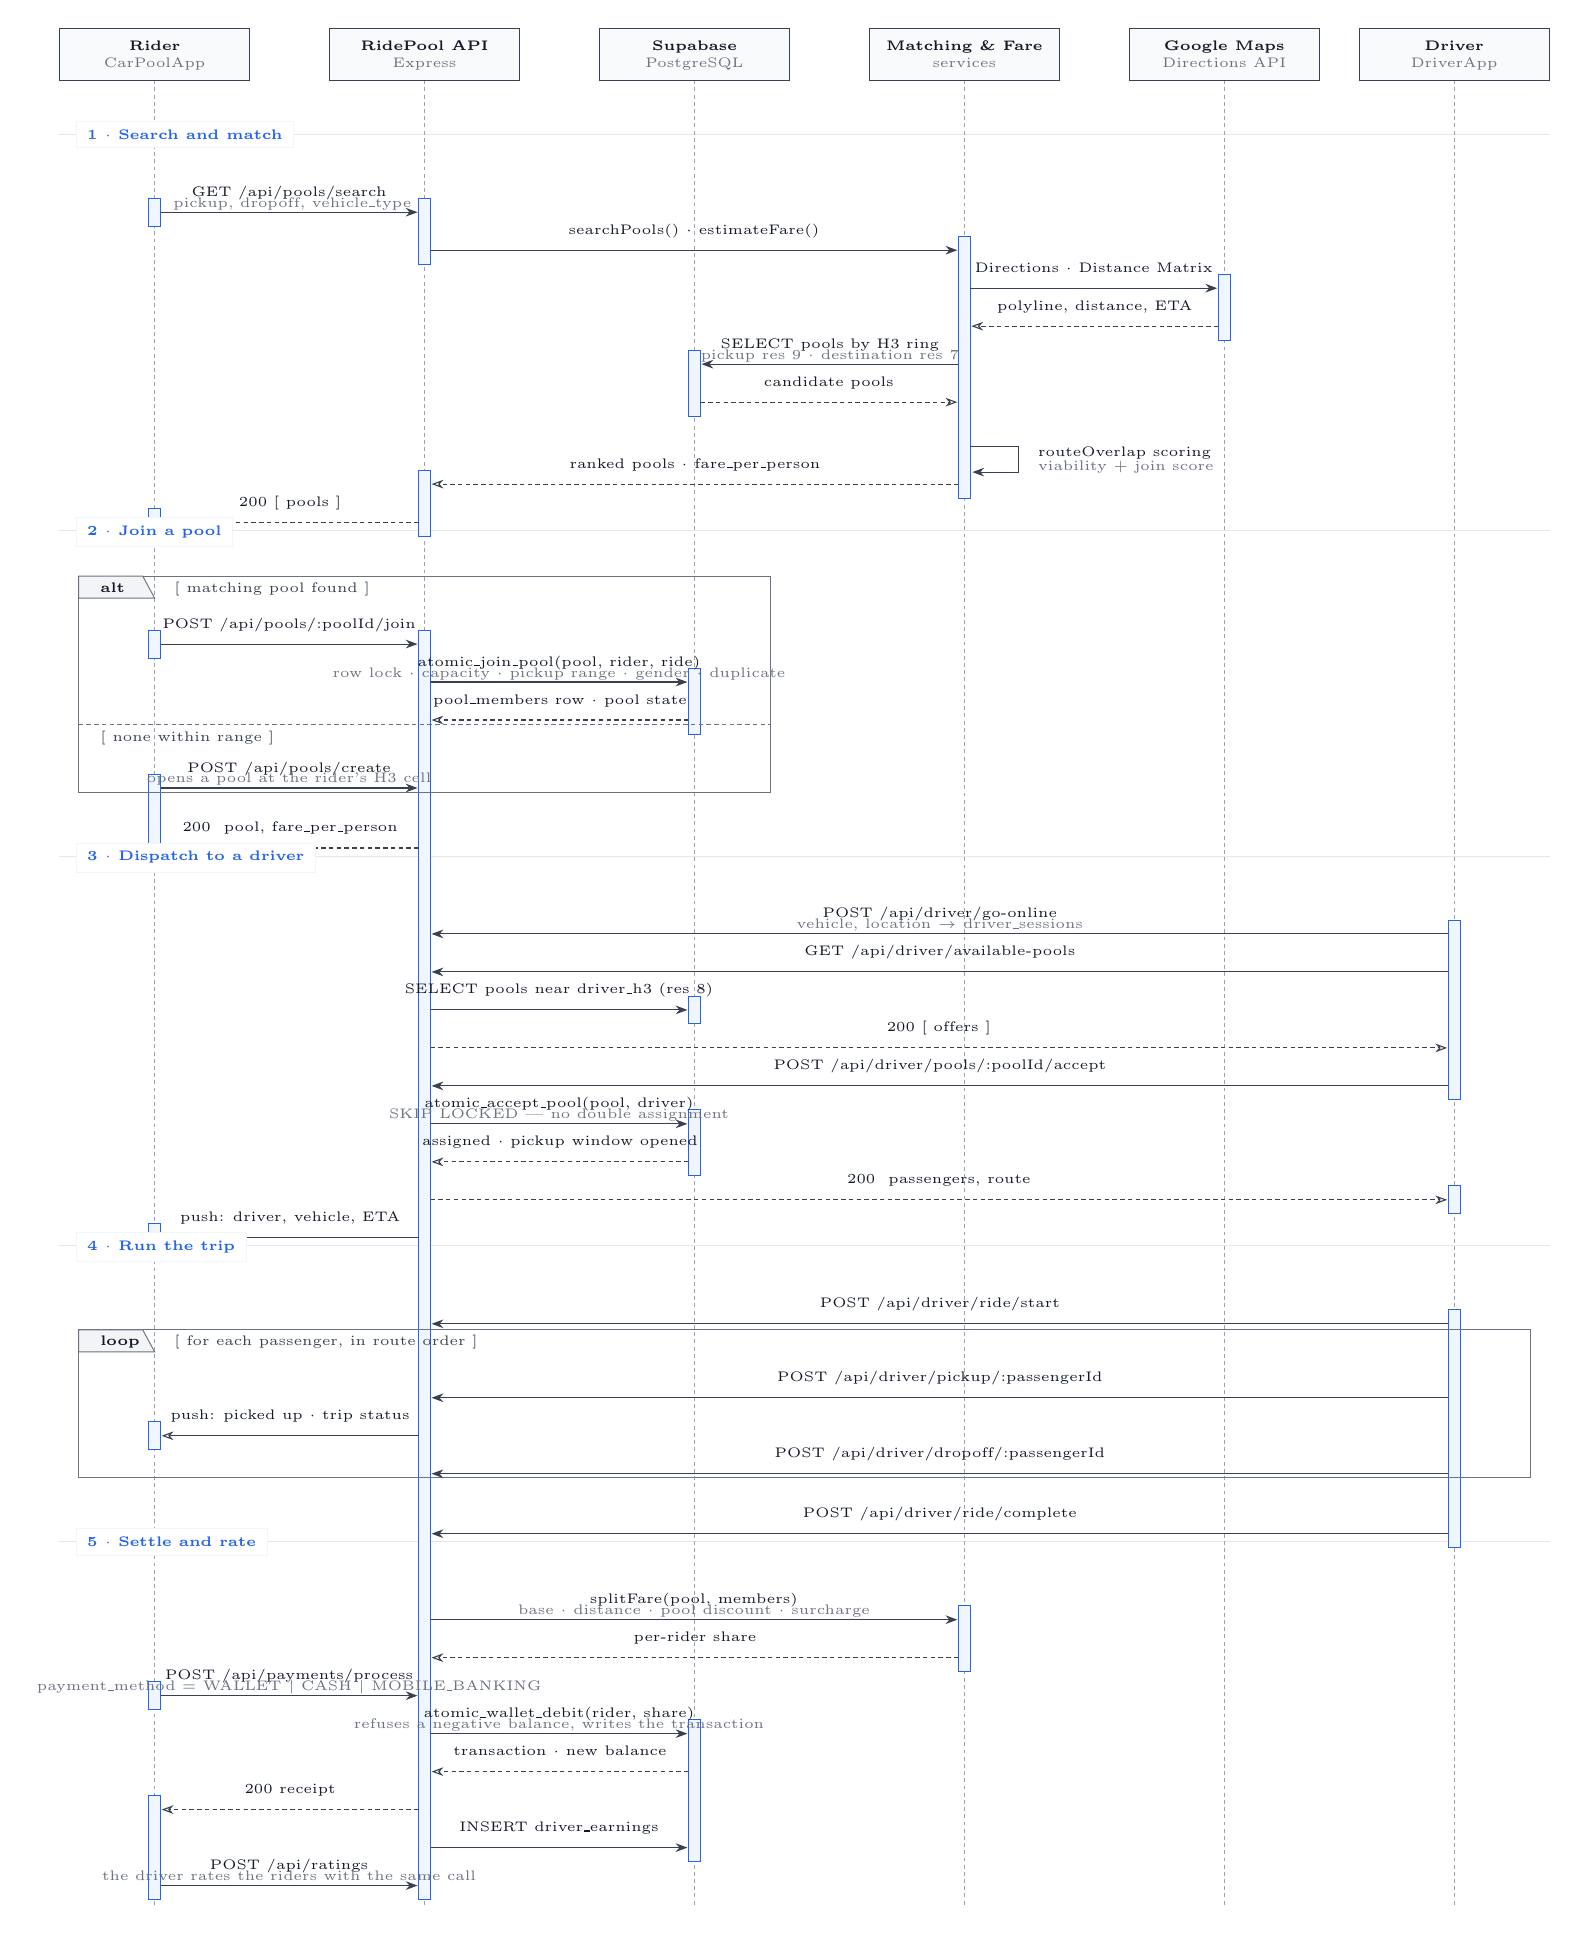
\begin{tikzpicture}[x=0.0127cm, y=-0.0127cm]

% ---------------- phase divider rules (labels come last) ----------------
\draw[draw=hairline, line width=0.3pt] (24,146) -- (1516,146);
\draw[draw=hairline, line width=0.3pt] (24,542) -- (1516,542);
\draw[draw=hairline, line width=0.3pt] (24,868) -- (1516,868);
\draw[draw=hairline, line width=0.3pt] (24,1258) -- (1516,1258);
\draw[draw=hairline, line width=0.3pt] (24,1554) -- (1516,1554);

% ---------------- lifelines ----------------
\draw[life] (120,92) -- (120,1920);
\draw[life] (390,92) -- (390,1920);
\draw[life] (660,92) -- (660,1920);
\draw[life] (930,92) -- (930,1920);
\draw[life] (1190,92) -- (1190,1920);
\draw[life] (1420,92) -- (1420,1920);

% ---------------- activation bars ----------------
\draw[draw=riderblue, line width=0.3pt, fill=riderbg] (114,210) rectangle (126,238);
\draw[draw=riderblue, line width=0.3pt, fill=riderbg] (114,520) rectangle (126,548);
\draw[draw=riderblue, line width=0.3pt, fill=riderbg] (114,642) rectangle (126,670);
\draw[draw=riderblue, line width=0.3pt, fill=riderbg] (114,786) rectangle (126,874);
\draw[draw=riderblue, line width=0.3pt, fill=riderbg] (114,1236) rectangle (126,1264);
\draw[draw=riderblue, line width=0.3pt, fill=riderbg] (114,1434) rectangle (126,1462);
\draw[draw=riderblue, line width=0.3pt, fill=riderbg] (114,1694) rectangle (126,1722);
\draw[draw=riderblue, line width=0.3pt, fill=riderbg] (114,1808) rectangle (126,1912);
\draw[draw=riderblue, line width=0.3pt, fill=riderbg] (384,210) rectangle (396,276);
\draw[draw=riderblue, line width=0.3pt, fill=riderbg] (384,482) rectangle (396,548);
\draw[draw=riderblue, line width=0.3pt, fill=riderbg] (384,642) rectangle (396,1912);
\draw[draw=riderblue, line width=0.3pt, fill=riderbg] (654,362) rectangle (666,428);
\draw[draw=riderblue, line width=0.3pt, fill=riderbg] (654,680) rectangle (666,746);
\draw[draw=riderblue, line width=0.3pt, fill=riderbg] (654,1008) rectangle (666,1036);
\draw[draw=riderblue, line width=0.3pt, fill=riderbg] (654,1122) rectangle (666,1188);
\draw[draw=riderblue, line width=0.3pt, fill=riderbg] (654,1732) rectangle (666,1874);
\draw[draw=riderblue, line width=0.3pt, fill=riderbg] (924,248) rectangle (936,510);
\draw[draw=riderblue, line width=0.3pt, fill=riderbg] (924,1618) rectangle (936,1684);
\draw[draw=riderblue, line width=0.3pt, fill=riderbg] (1184,286) rectangle (1196,352);
\draw[draw=riderblue, line width=0.3pt, fill=riderbg] (1414,932) rectangle (1426,1112);
\draw[draw=riderblue, line width=0.3pt, fill=riderbg] (1414,1198) rectangle (1426,1226);
\draw[draw=riderblue, line width=0.3pt, fill=riderbg] (1414,1322) rectangle (1426,1560);

% ---------------- combined fragments ----------------
\draw[frag] (44,588) rectangle (736,804);
\draw[frag, fill=fragbg] (44,588) -- (108,588) -- (120,610) -- (44,610) -- cycle;
\node[anchor=base west, font=\sqfrag, text=inkdark] at (56,604) {alt};
\node[anchor=base west, font=\sqguard, text=linegrey] at (130,604) {{[} matching pool found {]}};
\draw[frag, dash pattern=on 1.6pt off 1.2pt] (44,736) -- (736,736);
\node[anchor=base west, font=\sqguard, text=linegrey] at (56,753) {{[} none within range {]}};
\draw[frag] (44,1342) rectangle (1496,1490);
\draw[frag, fill=fragbg] (44,1342) -- (108,1342) -- (120,1364) -- (44,1364) -- cycle;
\node[anchor=base west, font=\sqfrag, text=inkdark] at (56,1358) {loop};
\node[anchor=base west, font=\sqguard, text=linegrey] at (130,1358) {{[} for each passenger, in route order {]}};

% ---------------- messages ----------------
\draw[call] (126,224) -- (383,224);
\node[anchor=base, font=\sqmsg, text=inkdark] at (254.5,208) {GET /api/pools/search};
\node[anchor=base, font=\sqsub, text=midgrey] at (254.5,219) {{ pickup, dropoff, vehicle\_type }};
\draw[call] (396,262) -- (923,262);
\node[anchor=base, font=\sqmsg, text=inkdark] at (659.5,246) {searchPools() $\cdot$ estimateFare()};
\draw[call] (936,300) -- (1183,300);
\node[anchor=base, font=\sqmsg, text=inkdark] at (1059.5,284) {Directions $\cdot$ Distance Matrix};
\draw[ret] (1184,338) -- (937,338);
\node[anchor=base, font=\sqmsg, text=inkdark] at (1060.5,322) {polyline, distance, ETA};
\draw[call] (924,376) -- (667,376);
\node[anchor=base, font=\sqmsg, text=inkdark] at (795.5,360) {SELECT pools by H3 ring};
\node[anchor=base, font=\sqsub, text=midgrey] at (795.5,371) {pickup res 9 $\cdot$ destination res 7};
\draw[ret] (666,414) -- (923,414);
\node[anchor=base, font=\sqmsg, text=inkdark] at (794.5,398) {candidate pools};
\draw[call] (936,458) -- (984,458) -- (984,484) -- (938,484);
\node[anchor=base west, font=\sqmsg, text=inkdark] at (994,468) {routeOverlap scoring};
\node[anchor=base west, font=\sqsub, text=midgrey] at (994,482) {viability + join score};
\draw[ret] (924,496) -- (397,496);
\node[anchor=base, font=\sqmsg, text=inkdark] at (660.5,480) {ranked pools $\cdot$ fare\_per\_person};
\draw[ret] (384,534) -- (127,534);
\node[anchor=base, font=\sqmsg, text=inkdark] at (255.5,518) {200 {[} pools {]}};
\draw[call] (126,656) -- (383,656);
\node[anchor=base, font=\sqmsg, text=inkdark] at (254.5,640) {POST /api/pools/:poolId/join};
\draw[call] (396,694) -- (653,694);
\node[anchor=base, font=\sqmsg, text=inkdark] at (524.5,678) {atomic\_join\_pool(pool, rider, ride)};
\node[anchor=base, font=\sqsub, text=midgrey] at (524.5,689) {row lock $\cdot$ capacity $\cdot$ pickup range $\cdot$ gender $\cdot$ duplicate};
\draw[ret] (654,732) -- (397,732);
\node[anchor=base, font=\sqmsg, text=inkdark] at (525.5,716) {pool\_members row $\cdot$ pool state};
\draw[call] (126,800) -- (383,800);
\node[anchor=base, font=\sqmsg, text=inkdark] at (254.5,784) {POST /api/pools/create};
\node[anchor=base, font=\sqsub, text=midgrey] at (254.5,795) {opens a pool at the rider's H3 cell};
\draw[ret] (384,860) -- (127,860);
\node[anchor=base, font=\sqmsg, text=inkdark] at (255.5,844) {200 { pool, fare\_per\_person }};
\draw[call] (1414,946) -- (397,946);
\node[anchor=base, font=\sqmsg, text=inkdark] at (905.5,930) {POST /api/driver/go-online};
\node[anchor=base, font=\sqsub, text=midgrey] at (905.5,941) {vehicle, location $\rightarrow$ driver\_sessions};
\draw[call] (1414,984) -- (397,984);
\node[anchor=base, font=\sqmsg, text=inkdark] at (905.5,968) {GET /api/driver/available-pools};
\draw[call] (396,1022) -- (653,1022);
\node[anchor=base, font=\sqmsg, text=inkdark] at (524.5,1006) {SELECT pools near driver\_h3 (res 8)};
\draw[ret] (396,1060) -- (1413,1060);
\node[anchor=base, font=\sqmsg, text=inkdark] at (904.5,1044) {200 {[} offers {]}};
\draw[call] (1414,1098) -- (397,1098);
\node[anchor=base, font=\sqmsg, text=inkdark] at (905.5,1082) {POST /api/driver/pools/:poolId/accept};
\draw[call] (396,1136) -- (653,1136);
\node[anchor=base, font=\sqmsg, text=inkdark] at (524.5,1120) {atomic\_accept\_pool(pool, driver)};
\node[anchor=base, font=\sqsub, text=midgrey] at (524.5,1131) {SKIP LOCKED --- no double assignment};
\draw[ret] (654,1174) -- (397,1174);
\node[anchor=base, font=\sqmsg, text=inkdark] at (525.5,1158) {assigned $\cdot$ pickup window opened};
\draw[ret] (396,1212) -- (1413,1212);
\node[anchor=base, font=\sqmsg, text=inkdark] at (904.5,1196) {200 { passengers, route }};
\draw[asyn] (384,1250) -- (127,1250);
\node[anchor=base, font=\sqmsg, text=inkdark] at (255.5,1234) {push: driver, vehicle, ETA};
\draw[call] (1414,1336) -- (397,1336);
\node[anchor=base, font=\sqmsg, text=inkdark] at (905.5,1320) {POST /api/driver/ride/start};
\draw[call] (1414,1410) -- (397,1410);
\node[anchor=base, font=\sqmsg, text=inkdark] at (905.5,1394) {POST /api/driver/pickup/:passengerId};
\draw[asyn] (384,1448) -- (127,1448);
\node[anchor=base, font=\sqmsg, text=inkdark] at (255.5,1432) {push: picked up $\cdot$ trip status};
\draw[call] (1414,1486) -- (397,1486);
\node[anchor=base, font=\sqmsg, text=inkdark] at (905.5,1470) {POST /api/driver/dropoff/:passengerId};
\draw[call] (1414,1546) -- (397,1546);
\node[anchor=base, font=\sqmsg, text=inkdark] at (905.5,1530) {POST /api/driver/ride/complete};
\draw[call] (396,1632) -- (923,1632);
\node[anchor=base, font=\sqmsg, text=inkdark] at (659.5,1616) {splitFare(pool, members)};
\node[anchor=base, font=\sqsub, text=midgrey] at (659.5,1627) {base $\cdot$ distance $\cdot$ pool discount $\cdot$ surcharge};
\draw[ret] (924,1670) -- (397,1670);
\node[anchor=base, font=\sqmsg, text=inkdark] at (660.5,1654) {per-rider share};
\draw[call] (126,1708) -- (383,1708);
\node[anchor=base, font=\sqmsg, text=inkdark] at (254.5,1692) {POST /api/payments/process};
\node[anchor=base, font=\sqsub, text=midgrey] at (254.5,1703) {payment\_method = WALLET $|$ CASH $|$ MOBILE\_BANKING};
\draw[call] (396,1746) -- (653,1746);
\node[anchor=base, font=\sqmsg, text=inkdark] at (524.5,1730) {atomic\_wallet\_debit(rider, share)};
\node[anchor=base, font=\sqsub, text=midgrey] at (524.5,1741) {refuses a negative balance, writes the transaction};
\draw[ret] (654,1784) -- (397,1784);
\node[anchor=base, font=\sqmsg, text=inkdark] at (525.5,1768) {transaction $\cdot$ new balance};
\draw[ret] (384,1822) -- (127,1822);
\node[anchor=base, font=\sqmsg, text=inkdark] at (255.5,1806) {200 receipt};
\draw[call] (396,1860) -- (653,1860);
\node[anchor=base, font=\sqmsg, text=inkdark] at (524.5,1844) {INSERT driver\_earnings};
\draw[call] (126,1898) -- (383,1898);
\node[anchor=base, font=\sqmsg, text=inkdark] at (254.5,1882) {POST /api/ratings};
\node[anchor=base, font=\sqsub, text=midgrey] at (254.5,1893) {the driver rates the riders with the same call};

% ---------------- phase labels, over what they cross ----------------
\node[anchor=base west, font=\sqphase, text=riderblue, fill=white, draw=riderbg,
      line width=0.3pt, inner xsep=4pt, inner ysep=3pt] at (41,151) {1 $\cdot$ Search and match};
\node[anchor=base west, font=\sqphase, text=riderblue, fill=white, draw=riderbg,
      line width=0.3pt, inner xsep=4pt, inner ysep=3pt] at (41,547) {2 $\cdot$ Join a pool};
\node[anchor=base west, font=\sqphase, text=riderblue, fill=white, draw=riderbg,
      line width=0.3pt, inner xsep=4pt, inner ysep=3pt] at (41,873) {3 $\cdot$ Dispatch to a driver};
\node[anchor=base west, font=\sqphase, text=riderblue, fill=white, draw=riderbg,
      line width=0.3pt, inner xsep=4pt, inner ysep=3pt] at (41,1263) {4 $\cdot$ Run the trip};
\node[anchor=base west, font=\sqphase, text=riderblue, fill=white, draw=riderbg,
      line width=0.3pt, inner xsep=4pt, inner ysep=3pt] at (41,1559) {5 $\cdot$ Settle and rate};

% ---------------- participants ----------------
\draw[draw=linegrey, line width=0.45pt, fill=sunken] (25,40) rectangle (215,92);
\node[anchor=base, font=\sqname, text=inkdark] at (120,62) {Rider};
\node[anchor=base, font=\sqrole, text=midgrey] at (120,79) {CarPoolApp};
\draw[draw=linegrey, line width=0.45pt, fill=sunken] (295,40) rectangle (485,92);
\node[anchor=base, font=\sqname, text=inkdark] at (390,62) {RidePool API};
\node[anchor=base, font=\sqrole, text=midgrey] at (390,79) {Express};
\draw[draw=linegrey, line width=0.45pt, fill=sunken] (565,40) rectangle (755,92);
\node[anchor=base, font=\sqname, text=inkdark] at (660,62) {Supabase};
\node[anchor=base, font=\sqrole, text=midgrey] at (660,79) {PostgreSQL};
\draw[draw=linegrey, line width=0.45pt, fill=sunken] (835,40) rectangle (1025,92);
\node[anchor=base, font=\sqname, text=inkdark] at (930,62) {Matching \& Fare};
\node[anchor=base, font=\sqrole, text=midgrey] at (930,79) {services};
\draw[draw=linegrey, line width=0.45pt, fill=sunken] (1095,40) rectangle (1285,92);
\node[anchor=base, font=\sqname, text=inkdark] at (1190,62) {Google Maps};
\node[anchor=base, font=\sqrole, text=midgrey] at (1190,79) {Directions API};
\draw[draw=linegrey, line width=0.45pt, fill=sunken] (1325,40) rectangle (1515,92);
\node[anchor=base, font=\sqname, text=inkdark] at (1420,62) {Driver};
\node[anchor=base, font=\sqrole, text=midgrey] at (1420,79) {DriverApp};

\end{tikzpicture}
% ============================= END FIGURE ============================
\end{document}

% =====================================================================
%  PLACING IT IN THE REPORT
%  Natural size is about 19.6 x 24.8 cm -- taller than a normal
%  text block. Give it its own page and fit it to the WIDTH (fitting to
%  \textheight would overflow the margins, since it is taller than it is wide):
%    \begin{figure}[p]\centering
%      \resizebox{\textwidth}{!}{\input{sequence-diagram-body}}
%      \caption{Sequence diagram for a pooled ride.}
%    \end{figure}
%  For larger text, split it at the "4 - Run the trip" divider into two
%  figures: phases 1-3 (request to dispatch) and phases 4-5 (trip to rating).
% =====================================================================
